\documentclass[a4paper]{article}

\usepackage{graphicx}
\usepackage{subfig}
\usepackage{multirow}
\usepackage[utf8]{inputenc}

\graphicspath{{figuras/}}

\hyphenation{ve-ri-fi-car FalaBrasil}

\title{Relatório 01}

\author{Pedro Batista (08080002701) - pedro@ufpa.br}

\begin{document}

\maketitle

\section{Projeto de Controladores PID}

\subsection{Controlador Proporcional}
A Equação~\ref{eq:exp1_sistema} mostra o sistema análisado nessa seção.
Primeiramente este foi simulado em malha aberta. A partir da
Figura~\ref{fig:exp1_aberta} é possível notar que o tempo de reposta
é extremamente lento ($t_r=252.8$), como esperado.

\begin{equation}
G_p=\frac{2}{1+100s}
\label{eq:exp1_sistema}
\end{equation}

Para reduzir o tempo de resposta, podemos adicionar um controlador proporcional
ao sistema. E de acordo com o critério de 2\%, sua constante de tempo deve
estar de acordo com as restrições da Equação~\ref{eq:tr_2p}.

\begin{equation}
\tau \leq \frac{tempo\_requerido}{4}
\label{eq:tr_2p}
\end{equation}

\begin{figure}[h]
   \subfloat[Sistema em malha aberta.]{\label{fig:exp1_aberta}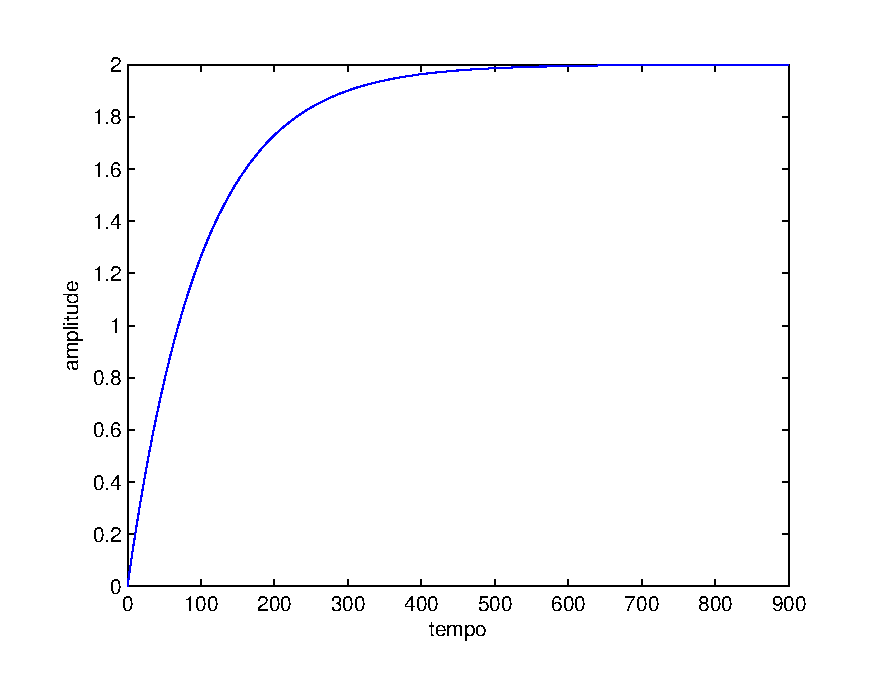
\includegraphics[width=0.5\textwidth]{exp1_aberta}}
   \caption{Gráficos gerados de acordo com a experiência 1, projeto de controlador
      proporcional.}
   \label{fig:primeira_ordem}
\end{figure}

\bibliographystyle{plain}
\bibliography{bib.bib} 
\end{document}
